\documentclass[../ClassicThesis.tex]{subfiles}
\begin{document}

% ************************************************
\chapter{Architecture}\label{ch:architecture}
% ************************************************

\newcommand\myNotes[1]{\textcolor{red}{#1}}

\section{Architecture Overview}
% ************************************************

\begin{figure}
  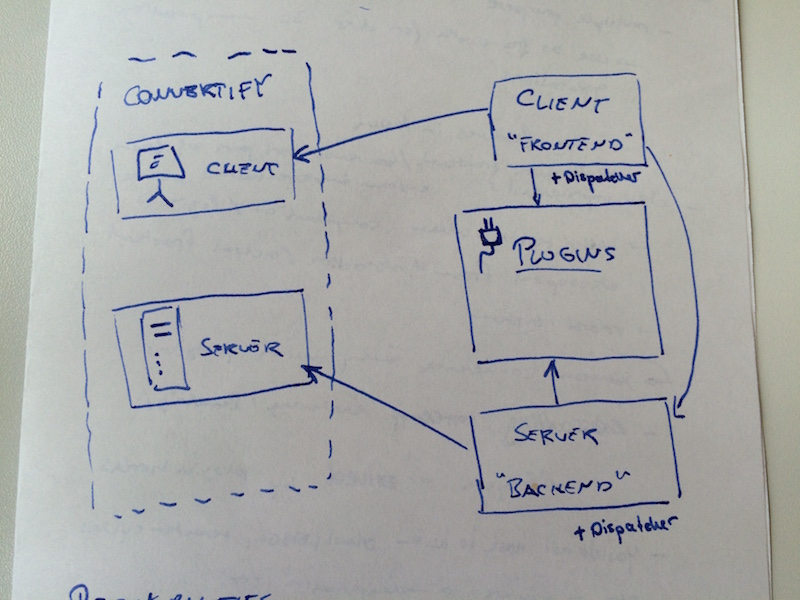
\includegraphics[width=1\columnwidth]{03-architecture_overview_current}
  \caption{Main Packages of the Platener Architecture}
  \label{fig:architectureOverviewCurrent}
\end{figure}

Platener is designed to enabled web-based manipulation and rendering of
{\threedmodel}s. Figure \ref{fig:architectureOverviewCurrent} shows the major
packages \emph{Convertify}, \emph{Client}, \emph{Server} and \emph{Plugins}. The
arrows indicate dependencies between the packages. The architecture emphasizes a
uni-directional data and event flow. Similar to mobile application design,
lifecycle events and the concept of
delegation\footnote{\url{https://developer.apple.com/library/ios/documentation/General/Conceptual/DevPedia-CocoaCore/Delegation.html}}
establish clear communication among packages.

% begin block comment
\iffalse
\begin{itemize}
\item platener built on top of...
\item 4 major packages: convertify, client, server and plugins
\item optimized towards: working with 3d-models in webgl environment
\item plugin-based: allow interchangeable computation logic/ conversion methods
\item combination of lifecycle-based communication and explicit calls via
  dispatchers (related work: mobile application design, mediator pattern) \ritem
  explicit communication between packages
\end{itemize}
\fi
% end block comment

\subsection{Package Responsibilities}

Each package takes over a set of distinct responsibilities ensuring decoupled
components. Thus a flexible, maintainable system is created.

\emph{Convertify} provides generic tools which support plugins in manipulating
{\threedmodel}s. This includes utilities for vector analysis as well as
rendering routines and scene management. The application lifecycle can be
initiated and observed via a \emph{Bundle}. A Bundle represents an instance of
the application's computation unit. The Client and Server packages run a Bundle.

\emph{Plugins} provide an exchangeable set of features which are used by the
Client and Server package. A Plugin interacts with the Scene and its
{\threedmodel}s via lifecycle events. E.g. a concrete conversion strategy
provided by Platener is implemented by a single Plugin. Plugin features can be
enabled for Client, Server or both.

The \emph{Client} package gives the look and feel of the application. This
package contains frontend components. The developer can choose any template
engine\footnote{\url{http://www.sitepoint.com/overview-javascript-templating-engines/}}
which serves the application's purpose. So the Client wires up the
{\userinterface} and the computation logic.

The \emph{Server} package is the headless counterpart to the Client package. A
Command Line Interface enables the user to run the application without a
browser. The Server also satisfies requests from the Client, such as caching and
loading models in a RESTful
interaction\footnote{\url{http://www.drdobbs.com/web-development/restful-web-services-a-tutorial/240169069}}.

% \begin{itemize}
% \item convertify: generic tools, helpers for 3d rendering, scene management,
%   model manipulation, platener independent
% \item client: look and feel, ux user interactions, wiring up/ firing up
%   computations, implemented for platener
% \item server: model storage/ cache, REST interaction, headless version of
%   client, CLI-tool chain, implemented for platener
% \item plugins: conversion specific computation and logic units, addons for
%   frontend and backend, platener independent
% \end{itemize}


\subsection{Decoupling the Framework into Packages}

Decoupling the software into packages builds a robust system. Computation logic
and UX components are kept apart, which allows isolated testing.

The Convertify package is meant to be used as a white-box framework for building
3D manipulation applications. Platener is such an application, supporting model
imports, rendering, altering and export of geometries. Introducing a web
framework makes sense, because WebGL gets more and more stable as of the year
2016 \myNotes{TODO: reference!}. Thus graphics software can be brought to huge
audience providing cross-platform web services.

% \begin{itemize}
% \item multpiple purpose:
% \item use as (whitebox) framework for other 3D manipulation applications (related work:
%   mechanism mining, etc)
% \item web service --> highly available, cross platform
% \item plug features in and out
% \item because concrete frontend/ backend not part of framework, custom
%   implementations possible (no vendor lock) \myNotes{this should be part of the
%     comparison with Brickify}
% \end{itemize}

Plugins are self-contained units which mainly interact with the WebGL scene and
its scene graph. Whole feature-sets can be switched on or off at once. They are
loosely coupled but have high cohesion at the same time. This prevents spaghetti
code and supports maintainability of each component. Furthermore, we use
software hooks to integrate plugins with rendering of models and access to
geometry data. This event-based approach allows developers to write a 3D
manipulation tool without having detailed domain knowledge about WebGL and
web-services. This will allows developers from the Computer Graphics domain to
concentrate on the graphics problem, rather than the web environment.

% \begin{itemize}
% \item dev improvements:
% \item better testing of computation/ logic because decoupled from ux
% \item robust system
% \item --> loose coupling of plugins, high cohesion in plugins
% \item --> isolated testing/ development possible
% \item solve cross-cuts: rendering/ loading <> lifecycle of plugins (eventbased)
% \item you do not have to know about WEBGL, render cycles etc. to provide a 3D
%   manipulation tool
% \item --> minimize web-domain knowledge as CG-devs are often unfamiliar with
%   this environment
% \end{itemize}

% \subsection{Discussion "vs Brickify"}

The Convertify package was not present in the Brickify architecture, see Figure
\ref{fig:architecture_overview_brickify}. This means Brickify provided a mix of
UX components, computation logic and interfacing code in the Client and Server
packages. Plugin communication was hard to observe and only implicitly ordered.
We introduced the new package to escape the vendor lock of previously used UX
libraries and to create a thoroughly testable code base.

\begin{figure}
\label{fig:architecture_overview_brickify}
  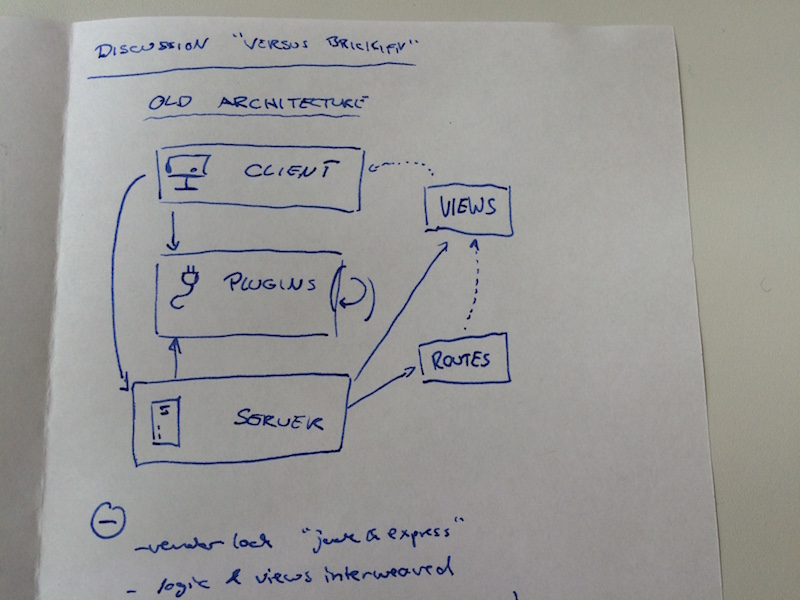
\includegraphics[width=1\columnwidth]{03-architecture_overview_brickify}
  \caption{Main Packages of the former Brickify Architecture}
\end{figure}

% \textbf{pros}
% \begin{itemize}
% \item fast enhancements as only views/ routes have to be adapted
% \item less interfacing because frontend <> logic tightly coupled
% \end{itemize}

% \textbf{cons}
% \begin{itemize}
% \item vendor lock: jade and express
% \item logic and views interweaved: high coupling --> hard testing, hard
%   maintainability, hard to change things
% \item implicit plugin communication
% \item complex management of custom 3d manipulation tools would require a lot of
%   rewrites because of view/ logic mix
% \end{itemize}

\section{Convertify Package and its Plugin Architecture}


\subsection{Convertify Purpose - Application Helpers}

\begin{itemize}
\item entry points
\item headless startup
\item basic logic for 3dmodel manipulation (import, mesh-conversion)
\item scenegraph and rendering (nodes, refs for sync objects in Brickify)
\item plugin interaction (hooks)
\item application helpers (threeHelper, renderHelper, commons (we should move
  commons to convertify))
\end{itemize}

\subsection{Render Lifecycle}

WHAT?

\begin{itemize}
\item App Lifecycle: Model Loading
\item Plugin Init
\item Scene Refreshes
\item Scene Graph Interactions
\item refer to Brickify
\end{itemize}

WHY?

\begin{itemize}
\item Gain control for computation units (plugins)
\item interact with the system
\end{itemize}

HOW?

\begin{itemize}
\item plugin hooks (refer to pluginHooks.yaml)
\item called on each plugin
\item allow plugin to handle the event (e.g do some manipulation to the scene)
\end{itemize}

\subsection{A Plugin is...}

WHAT?

\begin{itemize}
\item pluggable set of feature
\item or self-contained unit
\item can be activated for server/ client
\item composing multiple plugins --> extensible, maintainable method of building
  complex applications
\end{itemize}

WHY?

\begin{itemize}
\item Convertify as a framework
\item do not mix logic/ ui
\item decomposable logic (no spaghetti code)
\end{itemize}

HOW?

\begin{itemize}
\item define with package.json (could conceptionally be another npm package)
\item add to PluginMap
\item define hooks
\item space of freedom is huge...
\end{itemize}

\myNotes{see chapter ??, a list of plugins}
\myNotes{see chapters ?? for more detail}
\myNotes{maybe figure about lifecycle and hooks}

\subsection{Control Flow and Plugin Communication}

As Platener is composed of multiple plugins, which either represent computation
logic or render components, we have to know exactly when each of these plugins
will interact with the system. We propose a Dispatcher component, behaving
similar to the mediator
pattern\footnote{\url{https://sourcemaking.com/design_patterns/mediator}}.

\subsubsection{Dispatcher}

WHAT?

The Dispatcher is the entry point for any client or server code. The Dispatcher
loads and initializes a set of configured plugins. It organizes the
communication between plugins and client, plugins and server and plugins and
plugins in a single place.

\myNotes{reference figure}

% \begin{itemize}
% \item dispatcher is entry point for client -> logic, server -> logic
%   application
% \item loads and init given list of plugins via pluginloader
% \item implements each plugin hook and decides how to dispatch each call to the
%   plugins dependent on application state
% \end{itemize}

\textbf{events} Convertify fires lifecycle events on which the plugins can
react. The mediator knows an explicit execution order for each plugin when a
lifecycle event is fired.

\textbf{protocols}
\begin{itemize}
\item communication between packages (no lifecycle)
\item use protocols (explicit definition of what will happen)
\item protocol embodies a set of feature for the application
\end{itemize}

WHY?

\begin{itemize}
\item one guy who pulls all the strings (one source of truth)
\item similar designs in known application frameworks (android, ios)
\item javascript, non-type language --> protocols ensure correct interfaces
\end{itemize}

HOW?

\begin{itemize}
\item refer to Brickify, PluginLoader
\item explain plugins.yaml shortly
\item implements plugin hooks itself (show code snippets, hooks property)

\item implements protocols for plugins (show code snippets)
\item explain how plugins push state (control-flow information) back to the
  dispatcher
\end{itemize}

\begin{figure}
  \centering
  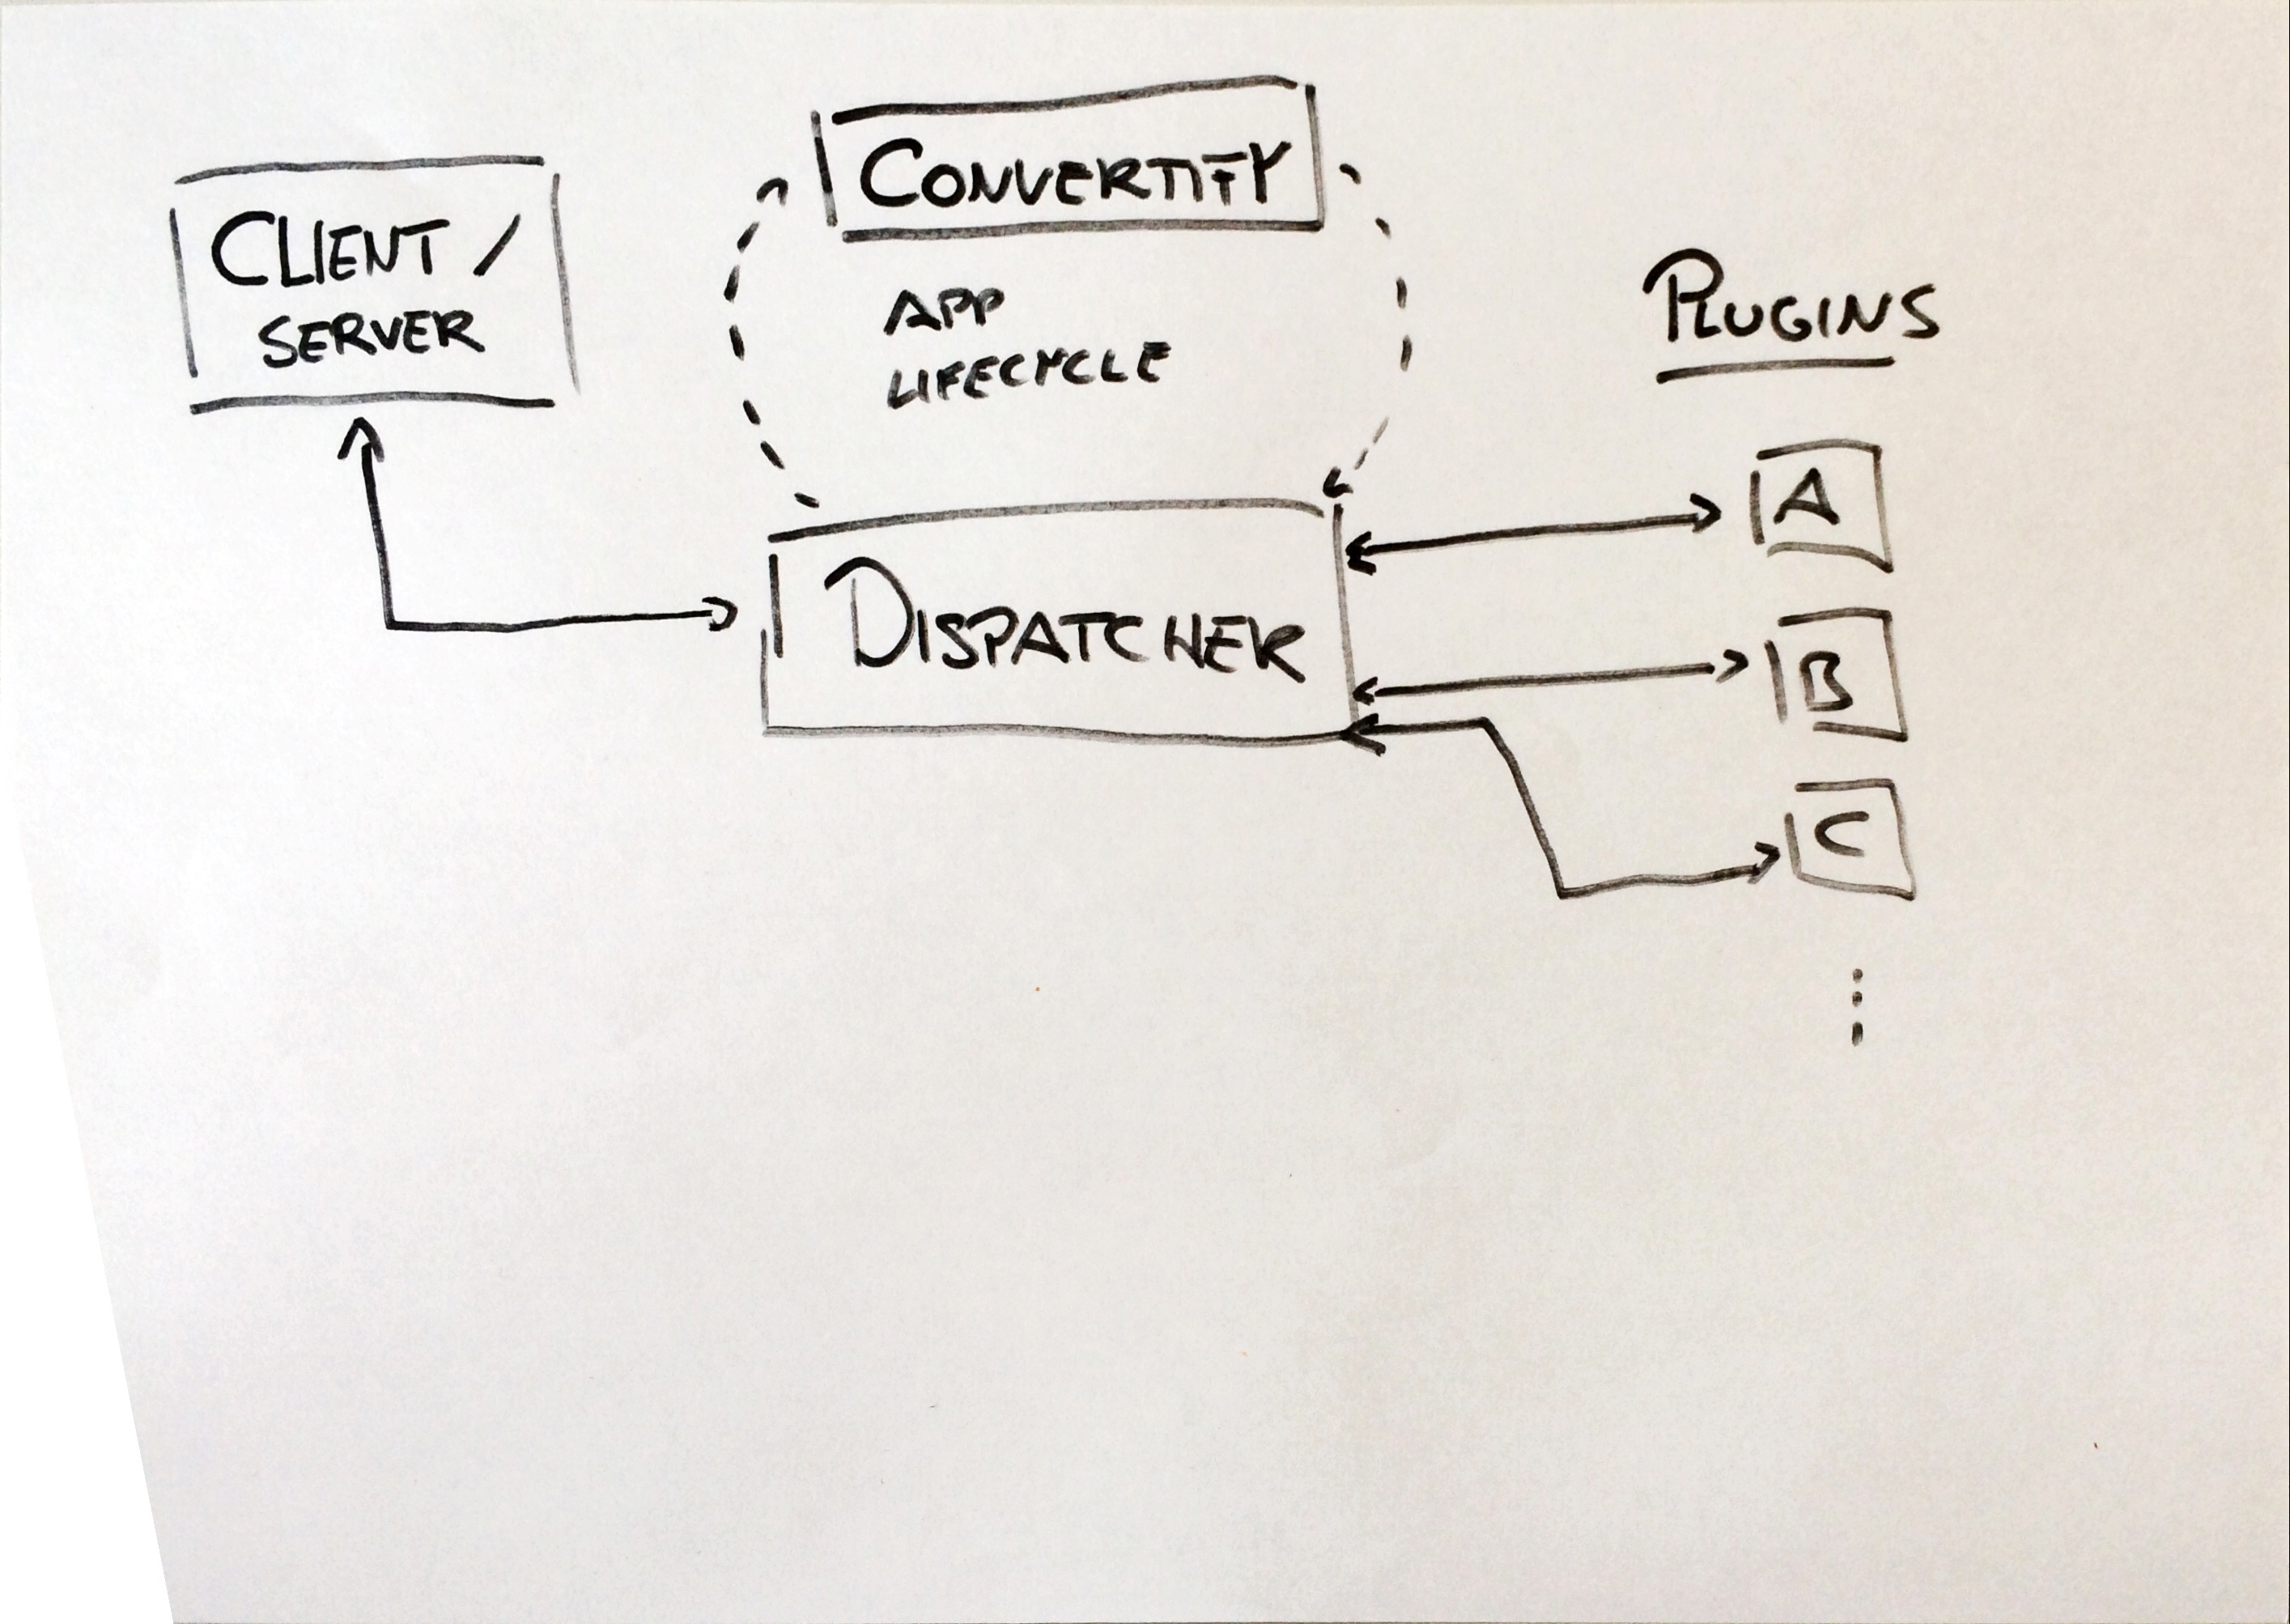
\includegraphics[width=1\columnwidth]{03-architecture_overview_dispatcher}
  \caption{Dispatcher manages inter-application communication during the
    lifecycle of the app.}
  \label{fig:architecture_overview_dispatcher}
\end{figure}


\subsubsection{Control Flow vs Brickify only plugin hooks}

\begin{itemize}
\item wiring up plugins
\item explicitly calling plugin hooks
\item highly customizable when adding in new plugins
\item how is control flow achieved? -->
\end{itemize}

\begin{itemize}
\item ++ pros
\item loading sequence control (impossible to repair)
\item fine grained scheduling of communication
\item explicit execution behavior
\item ... (look at notes on desk)
\item
\item -- cons
\item boilerplate code
\item custom integration for each plugin
\end{itemize}

\begin{itemize}
\item ++ pros
\item no further config needed
\item
\item -- cons
\item implicit order
\item in different use cases, different plugins have to interact first (order is
  not fixed)
\item frontend often has to work on data which is not available before another
  plugin loaded
\end{itemize}

\myNotes{now plugins can...}

\begin{itemize}
\item push application state back to the dispatcher
\item communication with each other by specifying a protocol which has to be
  implemented on the mediator
\item mediator then can oversee the communication
\end{itemize}

\section{Plugins}

\subsection{Plugin Overview}

% The Client package provides the look and feel of Platener. The Server package
% manages communication between frontend and data storage.

The plugins composed into Platener provides its computation logic and WebgGL
scene rendering. We will give a brief introduction of each plugin in the
following paragraphs.

\subsubsection{Coordinate System}

This plugin provides orientation enhancements for the WebGL scene. Rendering
xyz-axes and a an axis-aligned grid, users can grasp alignment and dimensions of
{\threedmodel}s. Figure \ref{fig:architecture_overview_coordinate_system} shows
the coordinate system in the WebGL view.

\begin{figure}
  \label{fig:architecture_overview_coordinate_system}
  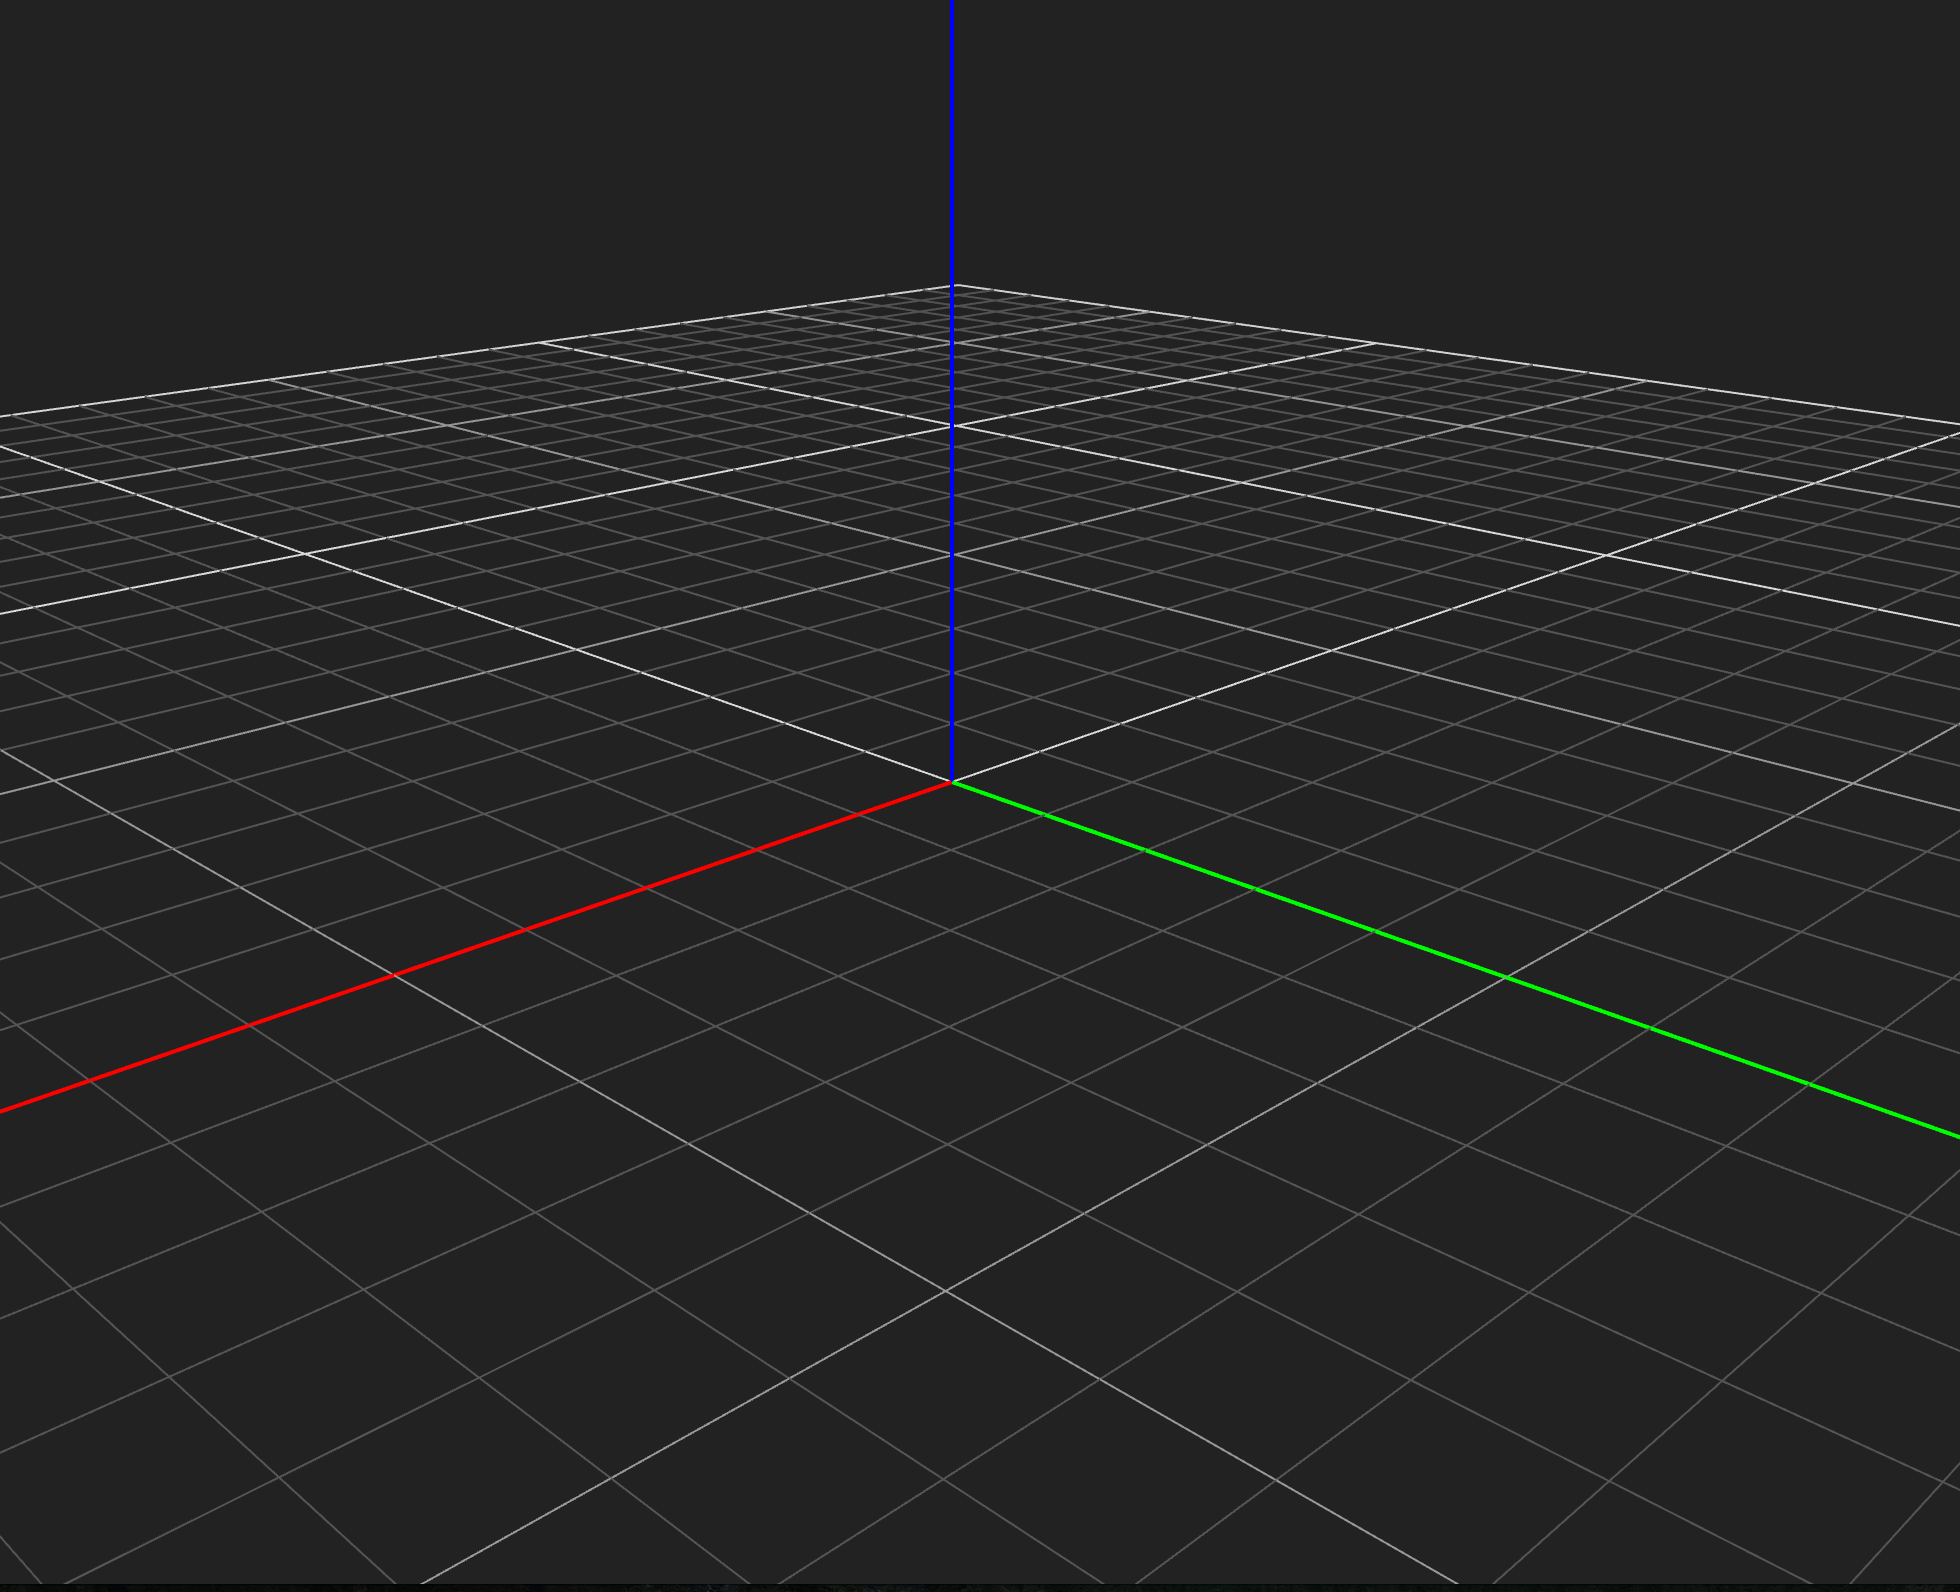
\includegraphics[width=1\columnwidth]{03-architecture_overview_coordinate_system}
  \caption{An empty scene showing the coordinate system.}
\end{figure}

\subsubsection{Platener Pipeline}

The Platener Pipeline plugin is the main computation unit. The plugin defines
multiple {\fabmethod}s. A {\fabmethod} is a conversion approach of a
\threedmodel. Multiple components, which can manipulate the input model, are
chained after another to produce 2D- or 3D-output. For example construction
plans for the original input model as {\svgfile}s.

\subsubsection{Node Visualizer}

We visualize the results of the Platener Pipeline plugin in the WebGL view. The
Node Visualizer plugin renders the results of each component of each
{\fabmethod} respectively.

\subsubsection{Scoring}

When multiple {\fabmethod}s are run, we want to choose the best fitted
conversion as output. Thus each {\fabmethod} is scored by a method-specific
scoring algorithm. This plugin provides these scoring algorithms.

\subsubsection{Solution Selection}

This plugin utilizes the Platener Pipeline plugin and the Scoring plugin to run
and evaluate all {\fabmethod}s. It outputs the result of the {\fabmethod} with
the best score and notifies the Dispatcher.

\subsubsection{Isolated Testing}

While we worked at different stages of a linearly executed {\fabmethod} in
parallel, we needed a mechanism to test each component of the {\fabmethod}
before its preceeding or succeeding components were finished. The Isolated
Testing plugin provides an isolated environment, which allows to execute a
single component of a {\fabmethod} with pre-defined input.

% - working in parallel, while needing inputs of work in progress - validate &
% visualize test scenarios for separate pipeline steps (components of a
% \fabmethod) - provide input for a given step and compute/ render results for
% just that step


\subsection{Platener Pipeline}

\begin{enumerate}
\item Overview/ Purpose/ Plugin Structure

\item \begin{itemize}
  \item conversion strategies and logic
  \end{itemize}

\item Pipeline Steps

  What are pipeline steps? Where to be found in the code? How are they used in
  Platener Pipeline?

\item Fabrication Methods


  \begin{enumerate}
  \item Plate Method


  \item Stacked Plates Method


  \item Classifier Method

  \end{enumerate}

\item Immutable Pipeline State


  \begin{enumerate}
  \item Overview/ Purpose


  \item Immutability


  \item Implementation Details

  \end{enumerate}
\end{enumerate}

\subsection{Node Visualizer}


\begin{enumerate}
\item Overview - Visual Debugging


\item Visualizer and Visualizations


\item Interwoven with Platener Pipeline


  \begin{enumerate}
  \item Role of Immutability


  \item Extracting Intermediate Data of the Pipeline

  \end{enumerate}
\end{enumerate}

\subsection{Isolated Testing}


\begin{enumerate}
\item Static Input and Expected Output


\item Testables

\end{enumerate}

\subsection{Scorer and Solution Selection}


Selecting the best estimated solution by default.

\section{Client Package}


\subsection{Overview - Custom Frontend Code}


\subsection{React Templates}


\subsection{Redux Data-driven Control Flow}


\begin{enumerate}
\item Dispatcher and Redux `dispatch`

\end{enumerate}

\section{Server Package}


\subsection{Overview - Custom Server Code}


\subsection{Model Cache}


\subsection{Test Pipeline}


\begin{enumerate}
\item Headless Conversion of Objects


\item Reports


\item Benchmarks

\end{enumerate}

\end{document}

%%% Local Variables:
%%% mode: latex
%%% TeX-master: "./03-Architecture"
%%% End:
